\documentclass[a4paper]{article}
\usepackage{graphicx}
\usepackage{wrapfig}
\usepackage{caption}
\usepackage{subcaption}


\title{Selection Sort}
\author{Yarne Ramakers}
\date{\today}

\begin{document}

%\maketitle - had to comment as it took up too much space
\begin{center}
  Insertion Sort \\
  Yarne Ramakers \\
  \today \\
\end{center}

\begin{figure}[h]
  \begin{subfigure}[b]{0.3\textwidth}
    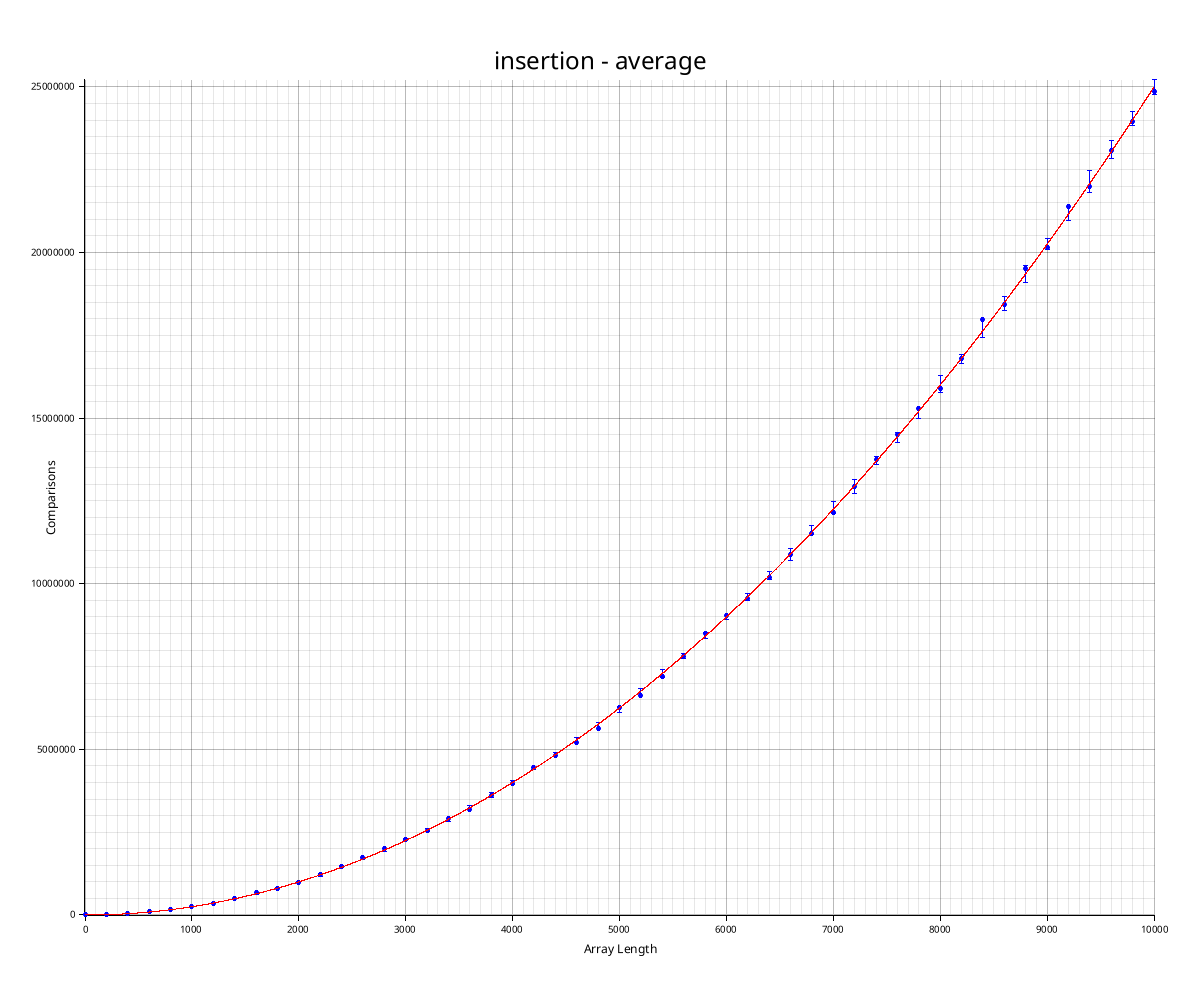
\includegraphics[width=\textwidth]{../out/insertion-average.png}
    \caption{Average case}
    \label{fig:insertion-avg}
  \end{subfigure}\hfill
  \begin{subfigure}[b]{0.3\textwidth}
    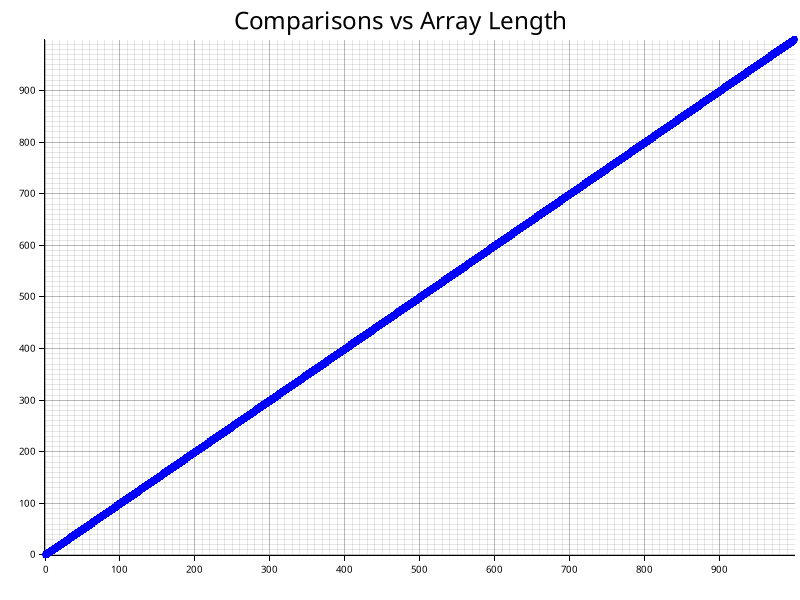
\includegraphics[width=\textwidth]{../out/insertion-best.png}
    \caption{Best case}
    \label{fig:insertion-best}
  \end{subfigure}\hfill
  \begin{subfigure}[b]{0.3\textwidth}
    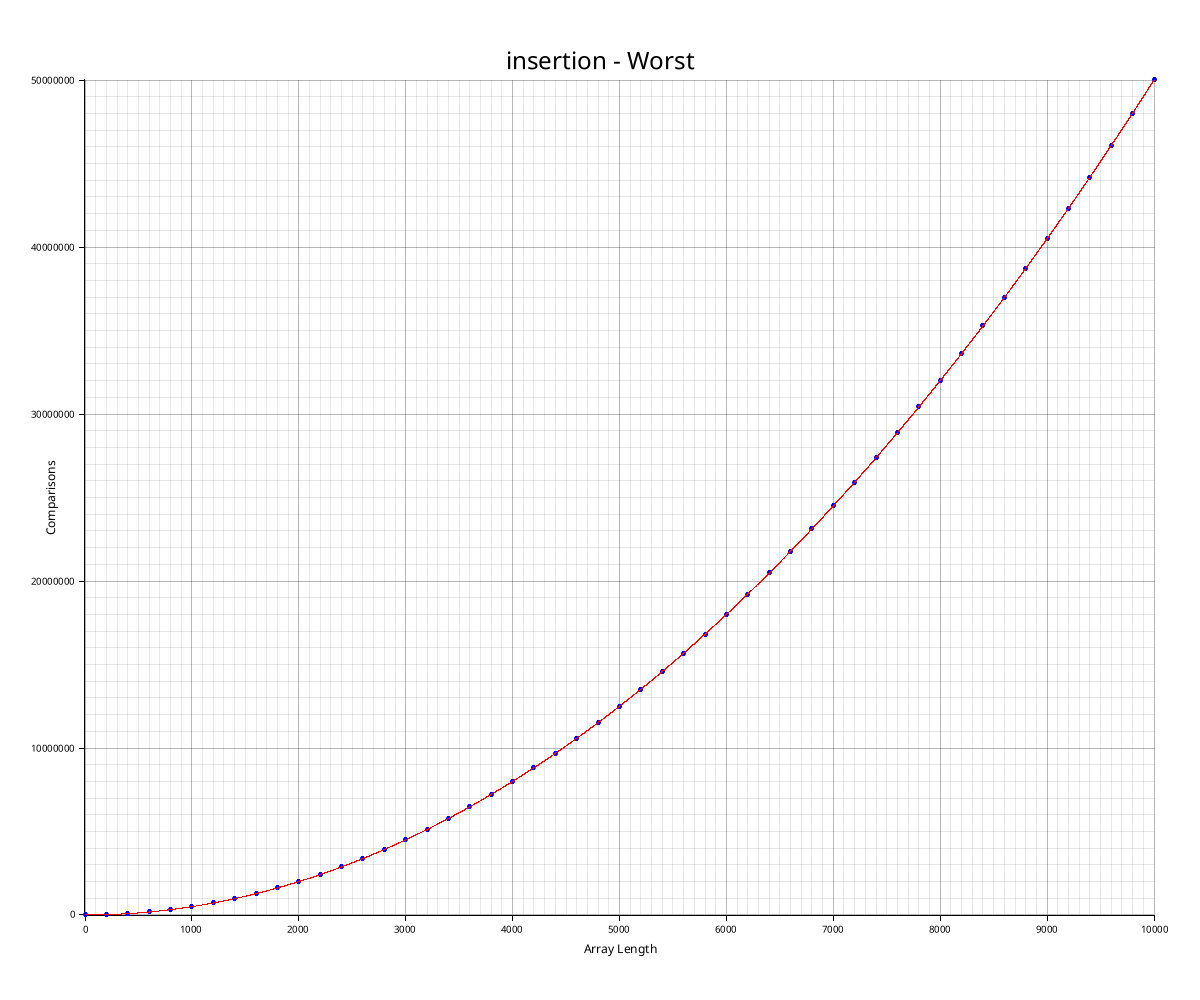
\includegraphics[width=\textwidth]{../out/insertion-worst.png}
    \caption{Worst case}
    \label{fig:insertion-worst}
  \end{subfigure}
\end{figure}

\section{Introductie}
% Introduction to inertion sort and its importance.

Insertion sort is een simpel sorteeralgoritme dat een lijst sorteert door een element uit de lijst te nemen en dit op de juiste plaats te zetten in de gesorteerde lijst.

\section{Bevindingen}
% Discuss the results of the experiments.
Mijn experimentele bevindingen vertonen sterke overeenkomsten met het theoretische model van insertion sort gezien in de les.
In de grafiek \ref{fig:insertion-avg} toont de rode lijn de theoretische complexiteit van selection sort, namelijk $\sim \frac{1}{4} n^2$. 
De blauwe punten tonen de gemeten vergelijkingen over lijsten voor verschillende lengte $n$. 
Deze $n$ is gekozen tussen 0 en 10 000 met een stapgrootte van 200, voor elke $n$ zijn er dan ook 5 metingen gebeurd. We merken op dat
de blauwe punten niet exact overeenkomen met de rode lijn, hiervoor is er dan ook een margelijn rond deze punten. Dit komt omdat insertion sort meer of minder vergelijkingen doet
afhankelijk van hoe de lijst al gesorteerd is. Als de lijst al partiëel gesorteerd is zal de complexiteit eerder naderen naar $\sim n$.
Als de lijst eerder in tegengestelde richting gesorteerd is zal de complexiteit naderen naar $\sim \frac{1}{2}n^2$. We merken wel op dat
het gemiddelde van die margelijn overeenkomt met de theoretische complexiteit.

\par

Voor lijsten met een kleinere $n$ is de gemeten complexiteit iets hoger dan de theoretische complexiteit.
Dit komt door de overhead van het meten van de complexiteit. Bij kleinere lijsten zullen de kleinere orde termen een grotere
invloed hebben op de gemeten complexiteit.

\par

Bij insertion sort maken we wel - in tegenstelling tot insertion sort - onderscheid tussen de cases. In best case scenario, wanneer de lijst al volledig gesorteerd is
moeten er enkel $n$ vergelijkingen gemaakt worden, omdat er nooit elementen verwisseld worden, en zal de complexiteit dus $\sim n$ zijn. Dit is te zien op grafiek \ref{fig:insertion-best}.
Is de lijst echter in tegengestelde richting gesorteerd, dan zal elk element elke keer volledig naar achter geschoven worden. Dit zal resulteren in een maximaal aantal vergelijkingen.
De complexiteit zal dan $\sim \frac{1}{2}n^2$ zijn. Dit is te zien op grafiek \ref{fig:insertion-worst}.

\end{document}